%*****************************************
\chapter{Multiple Sheets}\label{ch06:sheets}
%*****************************************
% Second pass corrections made and grammar checked 220624

Excel workbooks often contain a large amount of data, and worksheets can quickly become overwhelming. When one worksheet becomes cumbersome, data can be divided into smaller subsets and placed in separate worksheets within the same Excel file. Separating workbook data into smaller pieces can lead to better data organization within a file and increase its ease of use. For example, when a retail company needs to track overall sales and individual store sales, it makes sense to place each store's sales data in a separate worksheet within a file. Adding a worksheet that summarizes all the worksheets makes the data comprehensive. This chapter will show how to set up a workbook using multiple worksheets quickly and easily.

When spreading data across several worksheets, each worksheet must be laid out in the same way. A template facilitates this process. A template is a basic pattern for each new worksheet that can be used repeatedly to ensure each new worksheet has the same setup, formatting, and formulas. In this chapter, predefined Excel templates and those created from scratch will be used to meet the specific needs of the work required.

\section{Multiple Worksheet Basics}

\begin{center}
	\begin{objbox}{Learning Objectives}
		\begin{itemize}
			\setlength{\itemsep}{0pt}
			\setlength{\parskip}{0pt}
			\setlength{\parsep}{0pt}
			
			\item Navigating through a file with multiple worksheets.
			\item Adding, deleting, copying, and moving worksheets.
			\item Grouping and ungrouping worksheets.

		\end{itemize}
	\end{objbox}
\end{center}

The Excel workbooks used throughout this textbook have included multiple worksheets, so this concept will not be new. This chapter develops a personal budget file containing an entire year's income and expenses. The file contains a worksheet for each month of the year and a summary worksheet that totals all twelve monthly worksheets. The chapter begins with exercises designed to demonstrate organizing worksheets and ensuring that the monthly worksheets are consistently formatted. Figure \ref{06:fig01} shows the \textit{January} worksheet in the \textit{Personal Budget} file and all the worksheet tabs at the bottom of the window.

\begin{figure}[H]
	\centering
	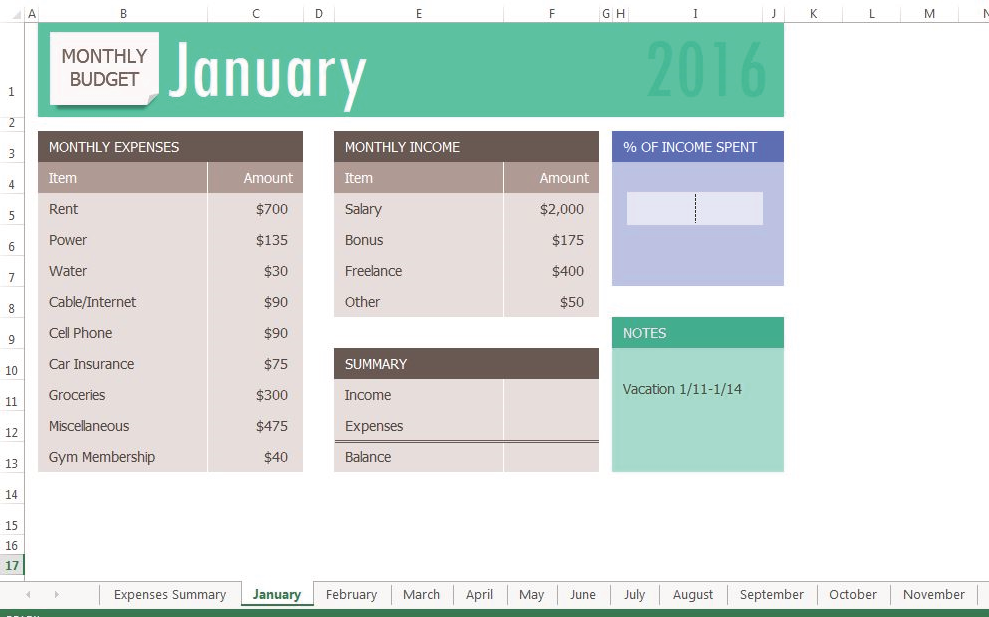
\includegraphics[width=\maxwidth{.95\linewidth}]{gfx/ch06_fig01}
	\caption{January Worksheet in the Personal Budget File}
	\label{06:fig01}
\end{figure}

\subsection{Navigating Through File with Multiple Worksheets}

\begin{enumbox}
	\begin{enumerate}
		\item Open \fmtWorksheet{CH6-Data} and save the file as \fmtWorksheet{CH6-Personal Budget}. Notice that the file has an \fmtWorksheet{Expenses Summary} worksheet tab at the far left followed by monthly worksheets.
		\item Click on the different worksheet tabs at the bottom of the screen to move through the worksheets. The \fmtWorksheet{Expenses Summary} worksheet is formatted differently from the monthly worksheets, but all the monthly worksheets are identical in layout and format.
		\item Take a second look at the months and notice the monthly expenses and income for September through October has not been added and there is no worksheet for December. 
		\item Add the following data in the \fmtWorksheet{September}, \fmtWorksheet{October}, and \fmtWorksheet{November} worksheets.
	\end{enumerate}
\end{enumbox}

\begin{table}[H]
	\rowcolors{1}{}{tablerow} % zebra striping background
	{\small
		%\fontsize{8}{10} \selectfont %Replace small for special font size
		\begin{longtable}{L{1.0in}L{0.75in}L{0.75in}L{0.75in}} %Left-aligned, Max width: 4.25in
			\textbf{Item} & \textbf{September} & \textbf{October} & \textbf{November} \endhead
			\hline
			Power         & $ \$135 $ & $ \$135 $ & $ \$135 $ \\
			Water         & $ \$30 $  & $ \$30 $  & $ \$30 $  \\
			Groceries     & $ \$300 $ & $ \$325 $ & $ \$400 $ \\
			Miscellaneous & $ \$100 $ & $ \$50 $  & $ \$100 $ \\
			Bonus         &           &           &           \\
			Freelance     & $ \$500 $ &           & $ \$150 $ \\
			Other         &           & $ \$100 $ &           \\

			\rowcolor{captionwhite}
			\caption{Data for September/October/November}
			\label{06:tab01}
		\end{longtable}
	}
\end{table}

\subsection{Copying a Worksheet}

To make a \textit{December} worksheet, copy the \textit{November} worksheet.

\begin{enumbox}
	\begin{enumerate}
		\item Point the mouse at the \fmtWorksheet{November} worksheet tab at the bottom of the screen.
		\item Press and hold the left mouse button and \fmtKeystroke{Ctrl} at the same time. 
		\item Drag the mouse to the right and drop the copied worksheet to the right of the \fmtWorksheet{November} worksheet.
		\item There should now be a \fmtWorksheet{November (2)} worksheet to the right of the \fmtWorksheet{November} worksheet as shown in Figure \ref{06:fig02}.

		\begin{figure}[H]
			\centering
			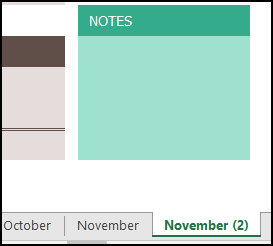
\includegraphics[width=\maxwidth{.50\linewidth}]{gfx/ch06_fig02}
			\caption{Additional November Worksheet}
			\label{06:fig02}
		\end{figure}

		\item Right-click on the \fmtWorksheet{November (2)} worksheet name at the bottom of the screen and choose \fmtButton{Rename}.
		\item Type \fmtTyping{December}, then tap \fmtKeystroke{Enter}.
		\item Click on the \fmtWorksheet{December} worksheet tab to activate it. Note, be sure to activate the cell and not just the \textit{Monthly Budget} image.
		\item Click cell \fmtLoc{B1} and change \textit{November} to \fmtTyping{December}.
		\item Make the following data changes.
	
		\begin{itemize}
			\item Miscellaneous: $ \$300 $
			\item Bonus: $ \$250 $ (holiday bonus)
			\item Freelance: delete amount
		\end{itemize}
		\item Save the \fmtWorksheet{CH6-Personal Budget} workbook.
		\item Point the mouse at the \fmtWorksheet{December} worksheet tab at the bottom of the screen.
		\item Press and hold the left mouse button and \fmtKeystroke{Ctrl} at the same time. 
		\item Drag the mouse to the right and drop the copied worksheet to the right of the \fmtWorksheet{December} worksheet.
		\item There should now be a \fmtWorksheet{December (2)} worksheet to the right of the \fmtWorksheet{December} worksheet.
		\item Rename the \fmtWorksheet{December(2)} worksheet to \fmtTyping{Practice}.
	\end{enumerate}
\end{enumbox}

\begin{center}
	\begin{sklbox}{Skill Refresher}
		\textbf{Copying a Worksheet}
		\\
		\begin{itemize}
			\setlength{\itemsep}{0pt}
			\setlength{\parskip}{0pt}
			\setlength{\parsep}{0pt}
			
			\item Point the mouse at the worksheet to copy at the bottom of the screen.
			\item Press and hold the left mouse button and \fmtKeystroke{Ctrl} at the same time.
			\item Drag the mouse to the right (still holding down the left-mouse button and \fmtKeystroke{Ctrl}) until the black down-pointing arrow is to the right of the existing worksheet.
			\item Let go of the mouse button and then \fmtKeystroke{Ctrl}. There should now be a \textit{Sheetname (2)} to the right of the original worksheet.
			\item Rename the \textit{Sheetname (2)} worksheet as desired.
			
		\end{itemize}
	\end{sklbox}
\end{center}

\subsection{Moving and Deleting Worksheets}

Sometimes worksheets are not in the correct order and need to be moved.

\begin{enumbox}
	\begin{enumerate}
		\item Point to the \fmtWorksheet{Practice} worksheet, then press and hold the left mouse button.
		\item Notice this time that there is still a black arrow to the left of the \fmtWorksheet{Practice} worksheet, but the piece of paper is blank. It does not have a plus sign ($ + $) because the worksheet is moving instead of copying.
		\item While still holding the left mouse button, drag to the left until a black arrow marker is between the \fmtWorksheet{October} and \fmtWorksheet{November} worksheets.
		\item Release the mouse button.
		\item Try moving the \fmtWorksheet{Practice} worksheet back to the right of the \fmtWorksheet{December} worksheet.
	\end{enumerate}
\end{enumbox}

Since the \textit{Practice} worksheet is unnecessary, use the following process to delete it.

\begin{enumbox}
	\begin{enumerate}
		\item Right-click on the \fmtWorksheet{Practice} worksheet tab at the bottom of the screen.
		\item Click \fmtButton{Delete}. Figure \ref{06:fig03} shows the warning message box that will appear, though it may look slightly different depending on the version of Excel being using. 
		\item Click \fmtButton{Delete}.
	\end{enumerate}
\end{enumbox}

\begin{figure}[H]
	\centering
	
\includegraphics[width=\maxwidth{.95\linewidth}]{gfx/ch06_fig03}
	\caption{Warning Message Box}
	\label{06:fig03}
\end{figure}

\begin{center}
	\begin{infobox}{Important!}
		\textbf{Deleting a Worksheet}
		\\
		\\
		Once a worksheet is deleted, \textit{Undo} will not bring it back, \textit{so be careful}.
	\end{infobox}
\end{center}

\subsection{Grouping and Ungrouping Worksheets}

Look at the monthly worksheets again. Notice there is a place in each of these worksheets to calculate three pieces of \textit{Summary} data: \textit{Income}, \textit{Expenses}, and \textit{Balance}, but there are no formulas in these cells. There is also a place for the \textit{\% of Income Spent}, but a formula is needed in $ I6 $ to calculate this. If these formulas were individually added to each of the twelve monthly worksheets, it would take a long time, and since this task is very repetitive, mistakes would likely be made along the way. By grouping all the monthly worksheets, the formulas are entered only once but appear in all the worksheets.

\begin{enumbox}
	\begin{enumerate}
		\item Tap the \fmtWorksheet{January} worksheet tab to make it active.
		\item Press and hold \fmtKeystroke{Shift}, then click on the \fmtWorksheet{December} worksheet tab to group them.
	\end{enumerate}
\end{enumbox}

All $ 12 $ worksheets are selected, which can be verified in two ways, as illustrated in Figure \ref{06:fig04}.

\begin{enumbox}
	\begin{enumerate}
		\item Selected worksheet tabs are in bold font at the bottom of the screen.
		\item The title bar at the top of the screen adds the word \textit{Group} to the end of the title.
	\end{enumerate}
\end{enumbox}

\begin{figure}[H]
	\centering
	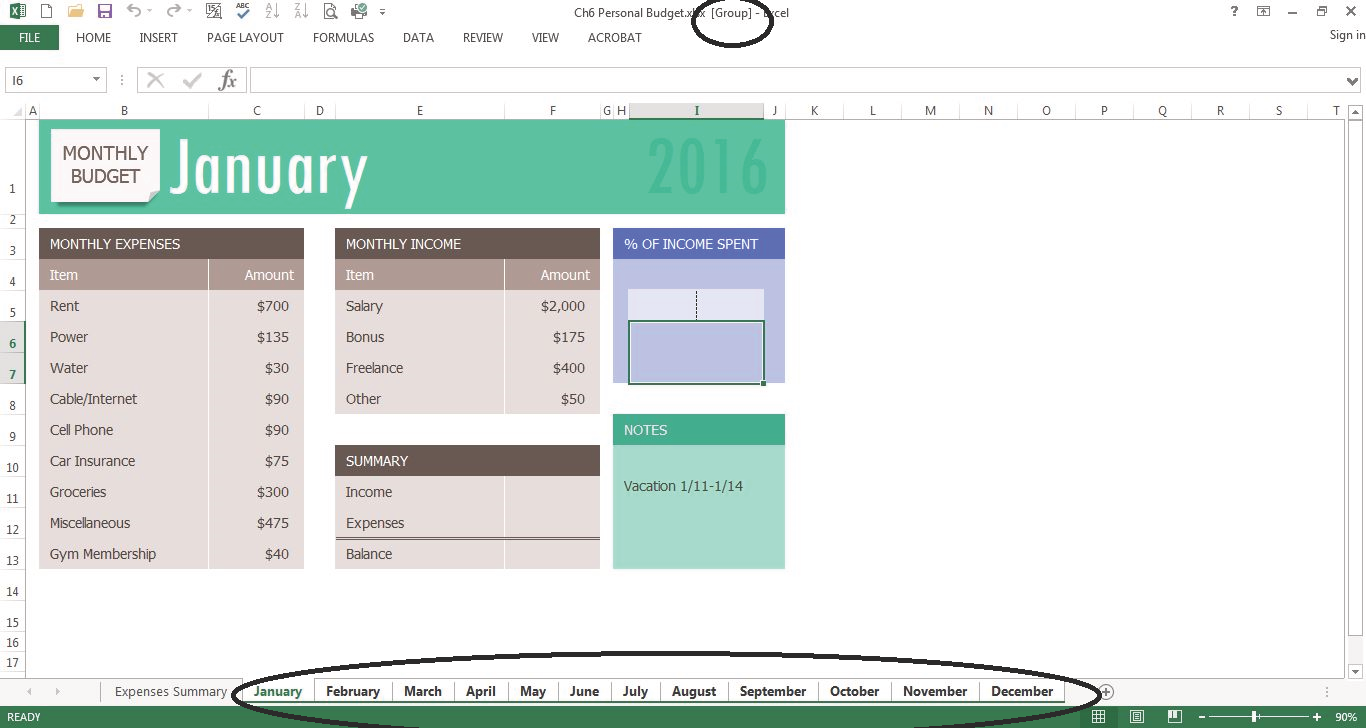
\includegraphics[width=\maxwidth{.95\linewidth}]{gfx/ch06_fig04}
	\caption{Grouped Worksheets}
	\label{06:fig04}
\end{figure}

\textit{It is important to remember that any changes made to the January worksheet will be made to all the grouped worksheets.} Grouping worksheets make it easy to make changes to all the worksheets at once, but they must be ungrouped after making changes, or data on linked worksheets can be inadvertently destroyed. 

\begin{enumbox}
	\begin{enumerate}
		\item Click cell \fmtLoc{F11} in the \fmtWorksheet{January} worksheet and enter the formula \fmtTyping{=SUM(F5:F8)}.
		\item In cell \fmtLoc{F12}, enter the formula \fmtTyping{=SUM(C5:C13)}.
		\item In cell \fmtLoc{F13}, subtract \textit{Expenses} from \textit{Income}. In the \fmtWorksheet{January} worksheet, the balance should be $ \$690 $. \textit{Hint}: if the answer is negative, then \textit{Income} was subtracted from \textit{Expenses} and the formula needs to be corrected.
		\item Click cell \fmtLoc{I6}. (\fmtLoc{I6} and \fmtLoc{I7} are merged, but that does not matter.)
		\item Enter a formula that divides \textit{Expenses} (\fmtLoc{F12}) by \textit{Income} (\fmtLoc{F11}). The answer will show as a percentage since this cell has already been formatted to do this. \textit{Hint}: If the percentage is greater than 100\% the numbers are reversed.
	\end{enumerate}
\end{enumbox}

Notice that a data bar was set up in $ I5 $ to visually show the income spent, a skill covered elsewhere in the course. The \textit{January} worksheet should now look like Figure \ref{06:fig05}.

\begin{figure}[H]
	\centering
	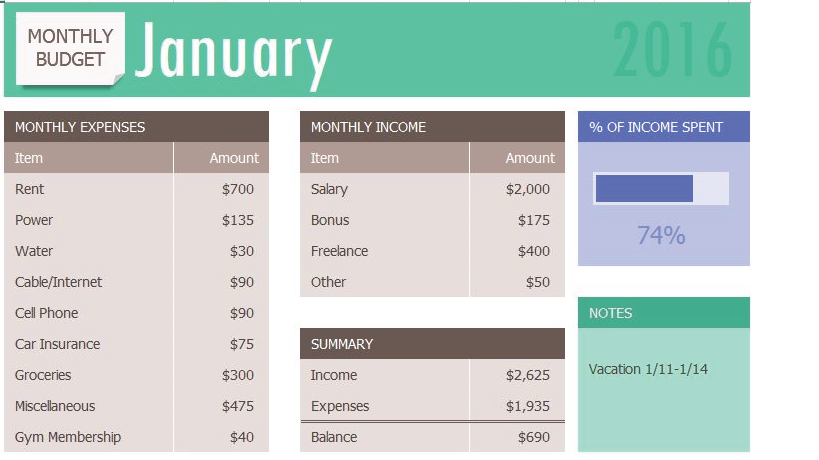
\includegraphics[width=\maxwidth{.95\linewidth}]{gfx/ch06_fig05}
	\caption{January Worksheet with Formulas}
	\label{06:fig05}
\end{figure}

\begin{enumbox}
	\begin{enumerate}
		\item Now that the monthly worksheets are done, they need to be ungrouped. Right-click on one of the grouped worksheet tabs and choose \fmtButton{Ungroup Sheets}. Notice the worksheets tabs are no longer bold and the word \textit{Group} is no longer in the title bar.
		\item Click on several of the month worksheets to see that all the formulas have been added.
		\item Click on the \fmtWorksheet{December} worksheet. The worksheet should look like Figure \ref{06:fig06}.
	\end{enumerate}
\end{enumbox}
	
\begin{figure}[H]
	\centering
	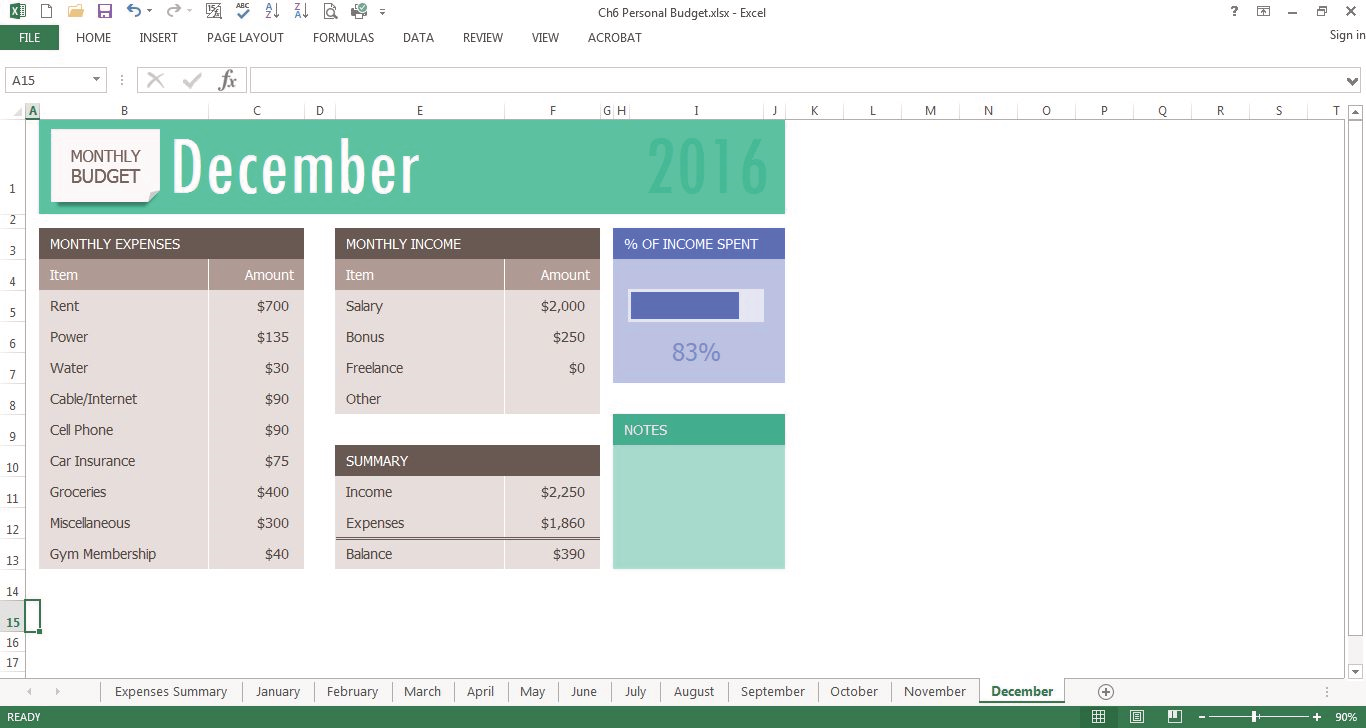
\includegraphics[width=\maxwidth{.95\linewidth}]{gfx/ch06_fig06}
	\caption{December Worksheet with Formulas}
	\label{06:fig06}
\end{figure}

Look at the \textit{Notes} in the \textit{September} worksheet. It says that the rent was raised in September, so the \textit{Gym Membership} needs to be canceled, and $ 0 $ should be entered for that amount in October, November, and December.

\begin{enumbox}
	\begin{enumerate}
		\item Group the \fmtWorksheet{October}, \fmtWorksheet{November}, and \fmtWorksheet{December} worksheets. If this is done successfully these three worksheet names should be bold and the word \textit{Group} will appear in the Title bar.
		\item Click the \fmtWorksheet{October} worksheet tab to activate it.
		\item Click cell \fmtLoc{C13} (\textit{Gym Membership}) and change the amount to $ \$0 $, then tap \fmtKeystroke{Enter}.
		\item Ungroup the worksheets. The \textit{Balance} should be October: $ \$605 $, November: $ \$530 $, and December: $ \$430 $.
		\item Save the \fmtWorksheet{CH6-Personal Budget} workbook.
	\end{enumerate}
\end{enumbox}

\begin{center}
	\begin{sklbox}{Skill Refresher}
		\textbf{To Group Worksheets}
		\\
		\begin{itemize}
			\setlength{\itemsep}{0pt}
			\setlength{\parskip}{0pt}
			\setlength{\parsep}{0pt}
			
			\item Click on the leftmost worksheet group.
			\item Press and hold \fmtKeystroke{Shift}, then click the rightmost worksheet to group.
		\end{itemize}
			
		\bigskip
			
		\textbf{To Ungroup Worksheets}
		\begin{itemize}
			\setlength{\itemsep}{0pt}
			\setlength{\parskip}{0pt}
			\setlength{\parsep}{0pt}
			
			\item Right-click on one of the grouped worksheets and choose \textit{Ungroup Worksheets}.
		\end{itemize}
	\end{sklbox}
\end{center}

\begin{center}
	\begin{tkwbox}{Key Take-Aways}
		\textbf{Worksheets}
		\\
		\begin{itemize}
			\setlength{\itemsep}{0pt}
			\setlength{\parskip}{0pt}
			\setlength{\parsep}{0pt}
			
			\item Worksheets can be easily moved, copied, deleted, and renamed.
			\item When grouped, identically formatted worksheets can be changed at the same time.
			
		\end{itemize}
	\end{tkwbox}
\end{center}

\section{Formulas With 3-D References}

\begin{center}
	\begin{objbox}{Learning Objectives}
		\begin{itemize}
			\setlength{\itemsep}{0pt}
			\setlength{\parskip}{0pt}
			\setlength{\parsep}{0pt}

			\item Entering formulas that reference another worksheet, which are called $ 3 $-D references.
			\item Using the SUM function to total values on multiple worksheets.
			
		\end{itemize}
	\end{objbox}
\end{center}

The \textit{Summary} worksheet presents totaled information from the other worksheets to give a quick synopsis in one convenient location. For this reason, the \textit{Summary} worksheet is usually the first worksheet in multiple-sheet files. Summary worksheets ``pull'' data from the other worksheets using three-dimensional ($ 3 $-D) cell references. A $ 3 $-D cell reference includes the worksheet name with the cell reference to distinguish between $ A3 $ in the \textit{Summary} worksheet and $ A3 $ in the monthly worksheets. The syntax to reference a cell in a different worksheet is \textit{=SheetName!CellRange}. So, the cell reference for $ A15 $ in the \textit{March} worksheet would be \textit{=March!A15}.

\begin{center}
	\begin{infobox}{Best Practice}
		\textbf{Summary Worksheet}
		\\
		\\
		Even if there are no $ 3 $-D formulas to summarize on a summary worksheet, it is considered a best practice to include a summary worksheet with information about the data contained in the workbook, the date the workbook was last updated, and contact information for the person who created the workbook.
	\end{infobox}
\end{center}

\subsection{Create the Expenses Summary Worksheet}

\begin{enumbox}
	\begin{enumerate}
		\item Click the \fmtWorksheet{Expenses Summary} worksheet tab to activate it.
		\item Click cell \fmtLoc{C5} and enter \fmtTyping{=January!C5}, then tap \fmtKeystroke{Enter}. This will get the amount $ \$700 $ from cell \fmtLoc{C5} in the \fmtWorksheet{January} worksheet.
		\item Delete the formula in \fmtLoc{C5} in the \fmtWorksheet{Expenses Summary} worksheet.
		\item This time, click cell \fmtLoc{C5} and type \fmtTyping{=}. Then click on the \fmtWorksheet{January} worksheet, click cell \fmtLoc{C5}, then tap \fmtKeystroke{Enter}.
		\item This will put the same formula, \fmtTyping{=January!C5}, in cell \fmtLoc{C5} in the \fmtWorksheet{Expenses Summary} worksheet and will return the value $ \$700 $. In general, it is more time-consuming to create a $ 3 $-D formula by clicking on separate worksheets, but it is less prone to error.
		\item In cell \fmtLoc{C6} in the \fmtWorksheet{Expenses Summary} worksheet, try entering a formula for the \textit{Power} amount in the \fmtWorksheet{April} worksheet. That amount should be $ \$135 $.
		\item Delete the formulas in cells \fmtLoc{C5} and \fmtLoc{C6} in the \fmtWorksheet{Expenses Summary} worksheet.
	\end{enumerate}
\end{enumbox}

For the \textit{Annual Amounts} in $ C5 $:$ C13 $ in the \textit{Expenses Summary} worksheet, the amount from a single month's worksheet is not needed; instead, the sum of all the entries in all the monthly worksheets should be entered. So, a $ 3 $-D sum for all twelve monthly worksheets should be entered. Here is a helpful hint on the steps that will sum cells on multiple worksheets.

\begin{center}
	\begin{sklbox}{Skill Refresher}
		\textbf{To SUM Across Worksheets}
		\\
		\begin{itemize}
			\setlength{\itemsep}{0pt}
			\setlength{\parskip}{0pt}
			\setlength{\parsep}{0pt}
			
			\item Click on the cell where the $ 3 $-D SUM should appear.
			\item Type \textit{=SUM(}
			\item Click on the leftmost worksheet in the group of worksheets to sum.
			\item Press and hold \fmtKeystroke{Shift}, then click the rightmost worksheet in the group of worksheets to sum.
			\item Click the cell in the worksheet that should be summed.
			\item Tap \fmtKeystroke{Enter}.
			
		\end{itemize}
	\end{sklbox}
\end{center}

Follow these steps to sum the monthly amounts in the \textit{Expenses Summary} worksheet.

\begin{enumbox}
	\begin{enumerate}
		\item Click cell \fmtLoc{C5} in the \fmtWorksheet{Expenses Summary} worksheet.
		\item Type \fmtTyping{=SUM(}. (Make sure to type the open parentheses.)
		\item Click on the \fmtWorksheet{January} worksheet.
		\item Press and hold \fmtKeystroke{Shift}, then click the \fmtWorksheet{December} worksheet.
		\item Click cell \fmtLoc{C5} again (this will be on the \fmtWorksheet{January} worksheet), then tap \fmtKeystroke{Enter}. Cell \fmtLoc{C5} should display the sum of $ \$8,400 $.
		\item Click on \fmtLoc{C5} in the \fmtWorksheet{Expenses Summary} worksheet. The formula bar should show the following: \fmtTyping{=SUM(January:December!C5)}. This means Excel will calculate the sum of \fmtLoc{C5} on the \fmtWorksheet{January} through \fmtWorksheet{December} worksheets.
		\item For another $ 3 $-D sum, click cell \fmtLoc{C6}.
		\item Type \fmtTyping{=SUM(}. (Make sure to type the open parentheses.)
		\item Click on the \fmtWorksheet{January} worksheet.
		\item Press and hold \fmtKeystroke{Shift}, then click the \fmtWorksheet{December} worksheet.
		\item Click cell \fmtTyping{C6} again, then tap \fmtKeystroke{Enter}. Cell \fmtLoc{C6} on the \fmtWorksheet{Expenses Summary} worksheet should now display the sum of $ \$1,610 $.
		\item Click cell \fmtLoc{C6} in the \fmtWorksheet{Expenses Summary} worksheet. The formula bar should show the following: \fmtTyping{=SUM(January:December!C6)}.
		\item Copy \fmtLoc{C6} to \fmtLoc{C7:C13}. The \fmtWorksheet{Expenses Summary} worksheet should match Figure \ref{06:fig07}.
		\item Save the \fmtWorksheet{CH6-Personal Budget} workbook.
	\end{enumerate}
\end{enumbox}

\begin{figure}[H]
	\centering
	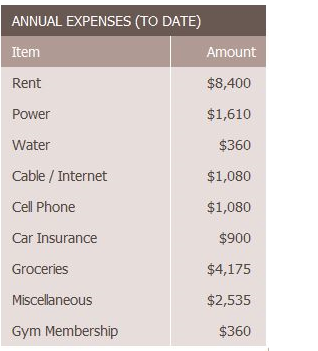
\includegraphics[width=\maxwidth{.95\linewidth}]{gfx/ch06_fig07}
	\caption{Complete Expenses Summary Formulas}
	\label{06:fig07}
\end{figure}

While the $ 3 $-D formulas are complete in the \textit{Expenses Summary} worksheet, the summary feels like it lacks something, so add a visual representation of the summary numbers to the worksheet.

\begin{enumbox}
	\begin{enumerate}
		\item Select cells \fmtLoc{B5:C13} in the \fmtWorksheet{Expenses Summary} worksheet.
		\item Click \fmtButton{Insert $ \Rightarrow $ Charts $ \Rightarrow $ Pie Chart $ \Rightarrow $ First 2-D Pie}.
	
		\item Resize the pie chart using the values below. •	For each side of the chart, press and hold \fmtKeystroke{Alt}, then left-click and drag the resize handle on the chart to make it ``lock into'' position.
	
		\begin{table}[H]
		\rowcolors{1}{}{tablerow} % zebra striping background
		\captionsetup{labelformat=empty} % kill the label and caption area
		{\small
			%\fontsize{8}{10} \selectfont %Replace small for special font size
			\begin{longtable}{R{0.75in}L{1.50in}} %Left-aligned, Max width: 4.25in
				\textbf{Chart Side} & \textbf{Locked To} \endhead
				\hline
				Top & Top of \fmtLoc{Row 3}\\
				Left & Left of \fmtLoc{Column D}\\
				Bottom & Bottom of \fmtLoc{Row 13}\\
				Right & Right of \fmtLoc{Column J}\\
			\end{longtable}
		} % End small
		\end{table}

		\item Click \fmtButton{Chart Design $ \Rightarrow $ Chart Layouts $ \Rightarrow $ Quick Layout $ \Rightarrow $ Layout $ 7 $}. That layout places the legend on the right side of the chart and removes the title (see Figure \ref{06:fig07a}).
	
		\begin{figure}[H]
			\centering
			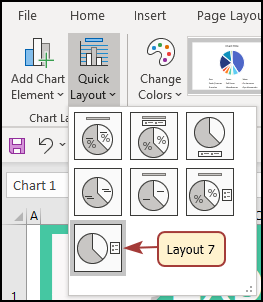
\includegraphics[width=\maxwidth{.60\linewidth}]{gfx/ch06_fig07a}
			\caption{Quick Layout Options}
			\label{06:fig07a}
		\end{figure}
	
		\item Click \fmtButton{Chart Design $ \Rightarrow $ Chart Layouts $ \Rightarrow $ Add Chart Element $ \Rightarrow $ Data Labels $ \Rightarrow $ Outside End}.
		\item The complete \fmtWorksheet{Expenses Summary} worksheet should look like Figure \ref{06:fig08} below.
		\item Save the \fmtWorksheet{CH6-Personal Budget} workbook. 
		\item Compare the workbook with the self-check answer key (\fmtWorksheet{CH6-Personal Budget Solution}) and then close and submit the \fmtWorksheet{CH6-Personal Budget} workbook as directed by the instructor.
	\end{enumerate}
\end{enumbox}
	
\begin{figure}[H]
	\centering
	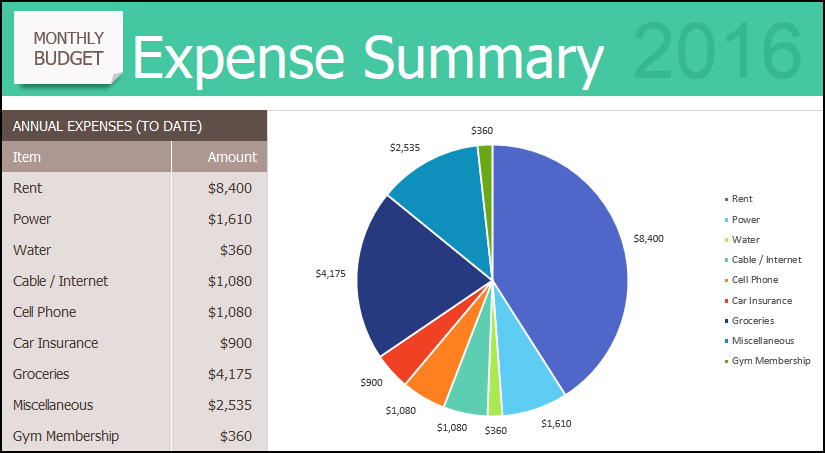
\includegraphics[width=\maxwidth{.95\linewidth}]{gfx/ch06_fig08}
	\caption{Completed Expenses Summary Worksheet}
	\label{06:fig08}
\end{figure}

\begin{center}
	\begin{sklbox}{Skill Refresher}
		\textbf{$ 3 $-D References in Formulas}
		\\
		\begin{itemize}
			\setlength{\itemsep}{0pt}
			\setlength{\parskip}{0pt}
			\setlength{\parsep}{0pt}
			
			\item To reference a cell in another worksheet, use the formula syntax \textit{=SheetName!CellAddress}.
			\bigskip
			\item To enter a $ 3 $-D reference:

			\begin{enumerate}
				\item Click on the cell where the formula should appear and type \textit{=}.
				\item Click the worksheet with the cell to reference.
				\item Click the cell, then tap \fmtKeystroke{Enter}.
			\end{enumerate}
			
		\end{itemize}
	\end{sklbox}
\end{center}

\begin{center}
	\begin{tkwbox}{Key Take-Aways}
		\textbf{3-D References}
		\\
		\begin{itemize}
			\setlength{\itemsep}{0pt}
			\setlength{\parskip}{0pt}
			\setlength{\parsep}{0pt}
			
			\item $ 3 $-D references in formulas allow data from one or more worksheets to be used on another worksheet.
			
		\end{itemize}
	\end{tkwbox}
\end{center}

\section{Templates}

\begin{center}
	\begin{objbox}{Learning Objectives}
		\begin{itemize}
			\setlength{\itemsep}{0pt}
			\setlength{\parskip}{0pt}
			\setlength{\parsep}{0pt}

			\item Use an existing Microsoft Excel template to create a new workbook.
			\item Create a custom template that can be used to create new workbook.
		
		\end{itemize}
	\end{objbox}
\end{center}

A template is a predefined pattern for a workbook. Hundreds of templates created by Microsoft are available to use inside Excel, which is beneficial to starting and completing a new task in Excel quickly. Templates include all the formulas and formatting needed in a professional Excel workbook. All that is left to do is enter the data. Predefined Microsoft templates include billing statements, blood pressure trackers, business cards, and many others. Categories include Business, Personal, Industry, Financial Management, Logs, Calculators, and Lists.

Sometimes a unique template is needed that is not predefined. Taking the time to create a custom template allows users to make standardized workbooks. This chapter explores both types of templates: predefined and custom.

\subsection{Predefined Templates}

Microsoft has made many predefined templates available in Excel. Follow these steps to explore this resource.

\begin{enumbox}
	\begin{enumerate}
		\item Click \fmtButton{File $ \Rightarrow $ New}.
		\item Click in the \textit{Search} box for Online template.
		\item Type \fmtTyping{Travel}, then tap \fmtKeystroke{Enter}.
		\item Click the \fmtButton{Travel Expense Report} and click \fmtButton{Create}. Note: If this template is not available, ask the instructor which template to use.
	\end{enumerate}
\end{enumbox}

The screen should look like Figure \ref{06:fig09} below. Notice that the design, layout, and formulas have already been set up.

\begin{figure}[H]
	\centering
	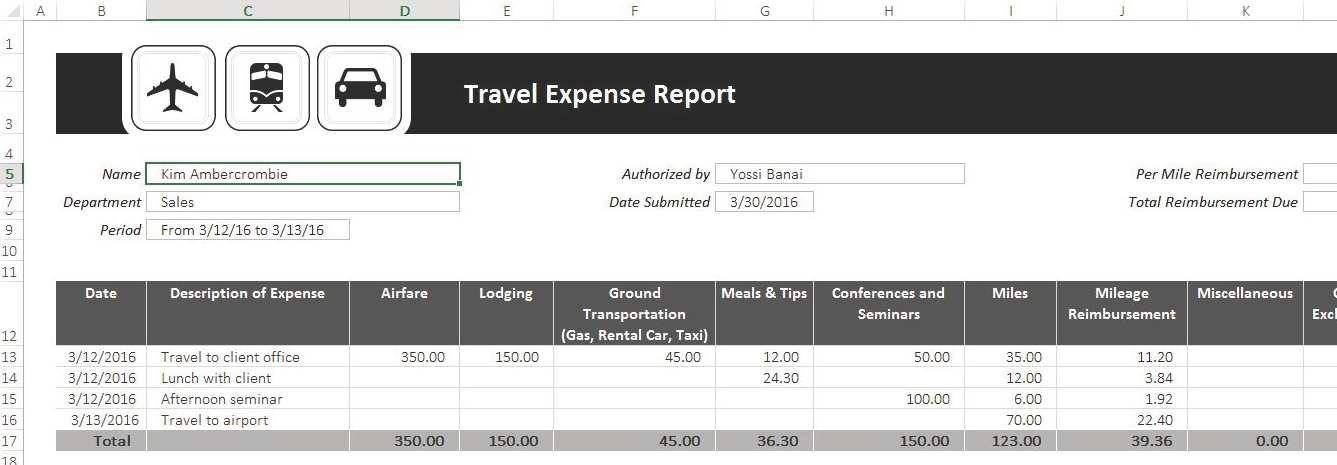
\includegraphics[width=\maxwidth{.95\linewidth}]{gfx/ch06_fig09}
	\caption{Travel Expenses Report Template}
	\label{06:fig09}
\end{figure}

Complete the following steps to investigate this template.

\begin{enumbox}
	\begin{enumerate}
		\item Enter the student's name in \fmtLoc{C3} (\textit{Name}).
		\item Enter \fmtTyping{CLL} in \fmtLoc{C5} (\textit{Department}).
		\item Press and hold \fmtKeystroke{Ctrl}, then tap \fmtKeystroke{$ \sim $} (that is \textit{Ctrl+tilde}) to see where the formulas are in the worksheet. Working in the formula view helps find formulas, so they will not be accidentally deleted.
		\item In formula view, carefully delete just the data in \fmtLoc{C10:I13}. Do not delete any formulas!
		\item Press and hold \fmtKeystroke{Ctrl}, then tap \fmtKeystroke{$ \sim $} (that is \textit{Ctrl+tilde}) again to return to Normal view.
		\item Enter dates and expenses for an imaginary trip in \fmtLoc{Row 10}, \fmtLoc{Row 11}, and \fmtLoc{Row 12}.
		\item Save the completed workbook as \fmtWorksheet{CH6-Travel Expenses}.
		\item Compare the workbook with the self-check answer key (\fmtWorksheet{CH6-Travel Expenses Solution}) and then close and submit the \fmtWorksheet{CH6-Travel Expenses} workbook as directed by the instructor.
	\end{enumerate}
\end{enumbox}

\begin{center}
	\begin{sklbox}{Skill Refresher}
		\textbf{Predefined Template}
		\\
		\begin{itemize}
			\setlength{\itemsep}{0pt}
			\setlength{\parskip}{0pt}
			\setlength{\parsep}{0pt}

			\item Click \textit{File $ \Rightarrow $ New}.
			\item Type the desired template description in the \textit{Search} box, then tap \fmtKeystroke{Enter}.
			
		\end{itemize}
	\end{sklbox}
\end{center}

\subsection{Custom Templates}

To create a custom template, either start with a blank workbook or use an existing workbook. Either way, the template can be used to create new workbooks that have a uniform appearance and set of functions. The existing \textit{CH6-Personal Budget} file will be converted into a template for this exercise. Other assignments in this chapter build a template from scratch.

\begin{enumbox}
	\begin{enumerate}
		\item Open the \fmtWorksheet{CH6-Personal Budget} file.
		\item Group the month worksheets (\fmtWorksheet{January} through \fmtWorksheet{December}).
		\item Press and hold \fmtKeystroke{Ctrl}, then tap \fmtKeystroke{$ \sim $} (that is \textit{Ctrl+tilde}) to switch to Formula view.
		\item Delete only the data from these worksheets, not labels or formulas. 
	
		\begin{itemize}
			\item Select \fmtLoc{C5:C13} (with all the worksheets still grouped), then tap \fmtKeystroke{Delete}.
			\item Select \fmtLoc{F5:F8} (with all the worksheets still grouped), then tap \fmtKeystroke{Delete}.
			\item Select \fmtLoc{H11:J13} (with all the worksheets still grouped), then tap \fmtKeystroke{Delete}.
		\end{itemize}	
	
	\item Press and hold \fmtKeystroke{Ctrl}, then tap \fmtKeystroke{$ \sim $} (that is \textit{Ctrl+tilde}) to switch back to Normal view.
		\item Ungroup the worksheets. 
		\item Look through the worksheets to check that only the data has been deleted. Notice the error message \textit{\#DIV/O} appears in \fmtLoc{I6} since the data for this formula has been deleted. The \fmtWorksheet{January} worksheet should look like Figure \ref{06:fig10}.
	\end{enumerate}
\end{enumbox}
	
\begin{figure}[H]
	\centering
	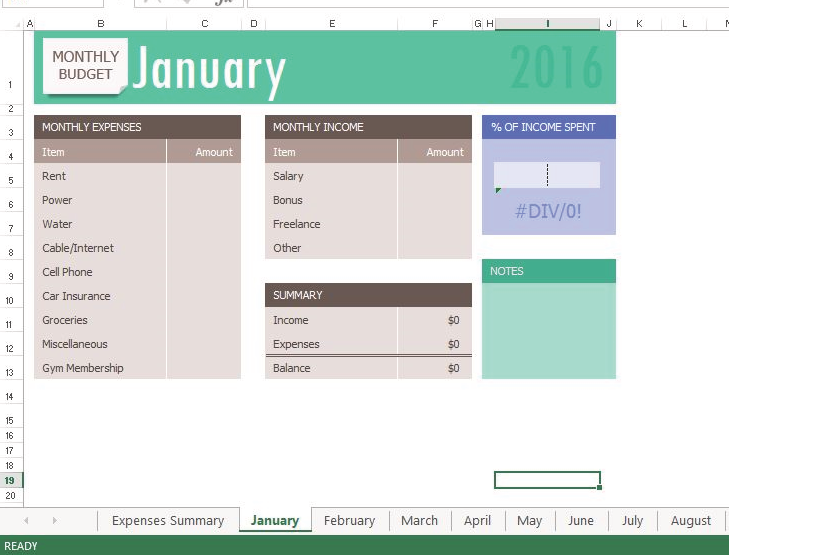
\includegraphics[width=\maxwidth{.95\linewidth}]{gfx/ch06_fig10}
	\caption{January Template Worksheet}
	\label{06:fig10}
\end{figure}

\textit{Note}: There are only formulas and the pie chart in the \textit{Expenses Summary} worksheet, so nothing needs to be deleted from this worksheet to set up the template.

\begin{enumbox}
	\begin{enumerate}
		\item Click \fmtButton{File $ \Rightarrow $ Save As}.
		\item Choose the location to save the file.
		\item In the \textit{Save as type} pull-down list, select \fmtButton{Excel Template (*.xltx)}.
		\item At the top of the screen, double-check that the location selected to save the file has not changed. If it has, navigate to the folder where the template will be saved. \textit{Be Careful Here!} By default, Excel will try to save this to a default template file location on the local hard drive.
		\item Type in the file name \fmtWorksheet{CH6-Personal Budget Template}. Carefully compare the screen with Figure \ref{06:fig11}. Keep in mind that the template file may be getting saved to a different place on the computer since Excel will normally save templates to a specific folder on the local hard drive.
		\item Click \fmtButton{Save}.
		\item Compare the workbook with the self-check answer key (\fmtWorksheet{CH6-Personal Budget Template Solution}) and then close and submit the \fmtWorksheet{CH6-Personal Budget Template} workbook as directed by the instructor.
	\end{enumerate}
\end{enumbox}
	
\begin{figure}[H]
	\centering
	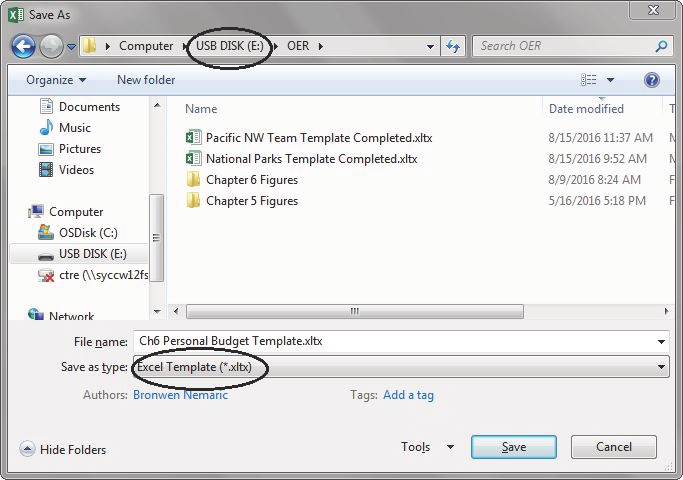
\includegraphics[width=\maxwidth{.95\linewidth}]{gfx/ch06_fig11}
	\caption{Save As Template}
	\label{06:fig11}
\end{figure}

\begin{center}
	\begin{sklbox}{Skill Refresher}
		\textbf{Save a Template}
		\\
		\begin{itemize}
			\setlength{\itemsep}{0pt}
			\setlength{\parskip}{0pt}
			\setlength{\parsep}{0pt}

			\item Click \textit{File $ \Rightarrow $ Save As}.
			\item Choose the location to save the file.
			\item In the \textit{Save as type} pull-down list, select \textit{Excel Template (*.xltx)}.
			\item At the top of the screen, double-check that the location to save the file to has not changed. If it has, navigate to the folder where the template will be saved. \textit{Be Careful Here!} By default, Excel will save templates to a default file location on the local hard drive.
			\item Enter the file name.
			\item Click \textit{Save}.
			
		\end{itemize}
	\end{sklbox}
\end{center}

Use the new budget template to start a Personal Budget file for $ 2017 $. 

\begin{enumbox}
	\begin{enumerate}
		\item Click \fmtButton{File $ \Rightarrow $ Open}.
		\item Navigate to the folder containing the \fmtWorksheet{CH6-Personal Budget Template} and open that file.
		\item Click \fmtButton{File $ \Rightarrow $ Save As}.
		\item Choose the location to save the $ 2017 $ version of the file.
		\item Change the \textit{Save as Type} to \fmtButton{Excel Workbook (*.xlsx)}.
		\item Enter the File name \fmtWorksheet{CH6-2017 Personal Budget}. Compare the screen to Figure \ref{06:fig12}.
	
		\begin{figure}[H]
			\centering
			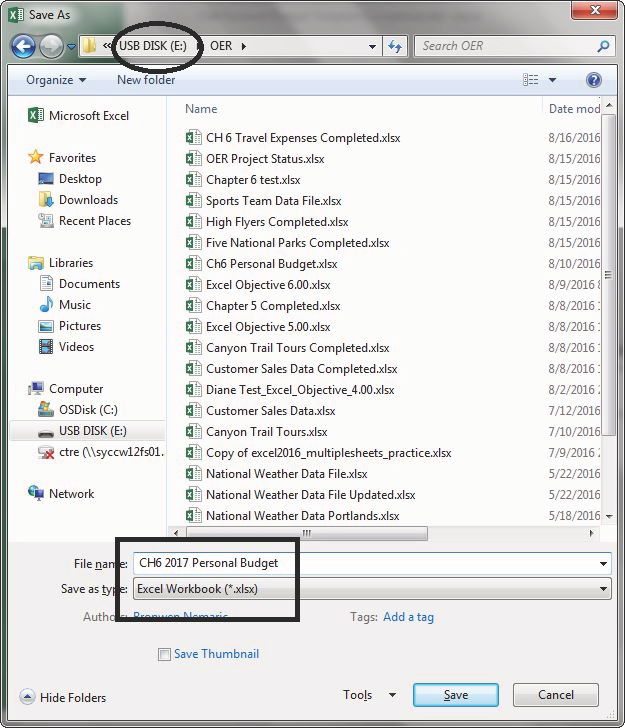
\includegraphics[width=\maxwidth{.95\linewidth}]{gfx/ch06_fig12}
			\caption{Save As 2017 Budget File}
			\label{06:fig12}
		\end{figure}

		\item Click \fmtButton{Save}.
		\item Group all the worksheets together including the \fmtWorksheet{Expenses Summary} worksheet.
		\item Click \fmtLoc{H1}. Type \fmtTyping{$ 2017 $}, then tap \fmtKeystroke{Enter}.
		\item Ungroup the worksheets.
		\item Click the \fmtWorksheet{January} worksheet tab to activate it. 
		\item Enter the data found in Figure \ref{06:fig13}.
	
		\begin{figure}[H]
			\centering
			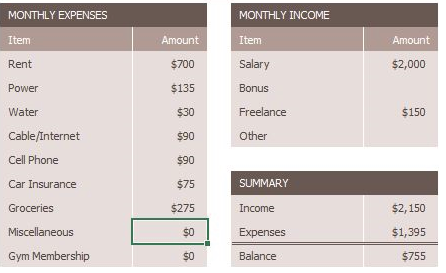
\includegraphics[width=\maxwidth{.95\linewidth}]{gfx/ch06_fig13}
			\caption{January 2017 Data}
			\label{06:fig13}
		\end{figure}

		\item Click the \fmtWorksheet{Expenses Summary} worksheet tab to activate it. The data and the pie chart should show the \textit{January} data since that is the only data in the twelve monthly worksheets. The worksheet should look like Figure \ref{06:fig14}.
		\item Save the \fmtWorksheet{CH6-2017 Personal Budget} workbook.
	\end{enumerate}
\end{enumbox}

\begin{figure}[H]
	\centering
	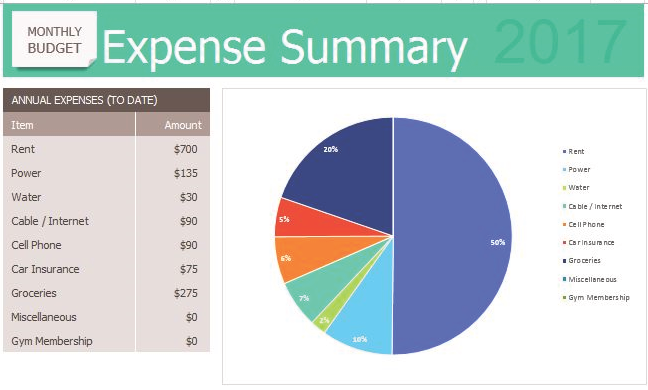
\includegraphics[width=\maxwidth{.95\linewidth}]{gfx/ch06_fig14}
	\caption{Expense Summary Worksheet}
	\label{06:fig14}
\end{figure}

\begin{center}
	\begin{tkwbox}{Key Take-Aways}
		\textbf{Templates}
		\\
		\begin{itemize}
			\setlength{\itemsep}{0pt}
			\setlength{\parskip}{0pt}
			\setlength{\parsep}{0pt}
			
			\item Templates save time and effort when compared to designing and creating workbook files from scratch.
			\item There are many predefined templates in Excel.
			\item Custom templates can be created for special purposes.
			
		\end{itemize}
	\end{tkwbox}
\end{center}

\section{Preparing to Print}

\begin{center}
	\begin{objbox}{Learning Objectives}
		\begin{itemize}
			\setlength{\itemsep}{0pt}
			\setlength{\parskip}{0pt}
			\setlength{\parsep}{0pt}
			
			\item Printing all the worksheets in a workbook at one time.
			\item Preparing multiple worksheets for printing using grouping.
			
		\end{itemize}
	\end{objbox}
\end{center}

Consistency in page setup is essential when working with workbooks containing multiple worksheets. Now that the \textit{2017 Personal Budget} workbook is complete prepare it for printing by changing the page orientation and adding a header. All $ 13 $ worksheets will also be printed at one time.

\subsection{Applying Page Setup Options to Grouped Worksheets}

As always, review the workbook in Print Preview before considering it complete.

\begin{enumbox}
	\begin{enumerate}
		\item Click \fmtButton{File $ \Rightarrow $ Print}.
		\item To view all the worksheets at one time, select \fmtButton{Print Entire Workbook} in the first box in the \textit{Settings} section. There should be $ 26 $ pages to scroll through in \textit{Print Preview}. At this point, clicking the \fmtButton{Print} button would print all the worksheets rather than just the active sheet.
		\item Exit \textit{Print Preview} by clicking the arrow button in the top left corner of the screen. The page orientation of all the worksheets can be changed at one time, but not in \textit{Print Preview}.
		\item Group all the worksheets together, including the \fmtWorksheet{Expenses Summary} worksheet through the \fmtWorksheet{December} worksheet.
		\item Click \fmtButton{Page Layout $ \Rightarrow $ Page Setup $ \Rightarrow $ Orientation $ \Rightarrow $ Landscape}.
		\item Click \fmtButton{Page Layout $ \Rightarrow $ Page Setup Launcher $ \Rightarrow $ Header/Footer Tab $ \Rightarrow $ Custom Footer}.
		\item In the center section of the custom footer, insert the worksheet name using the \fmtButton{Insert Sheet Name} button (that is the last button in the fourth group; it looks like a tiny worksheet). The Footer dialog box should look like Figure \ref{06:fig15}.
		\item Click \fmtButton{OK} to close the \textit{Footer} dialog box. Click \fmtButton{OK} again to close the \textit{Page Setup} dialog box.
		\item Click \fmtButton{File $ \Rightarrow $ Print} to return to \textit{Print Preview}. Check to see if each worksheet is printing on one page, in landscape orientation, with the correct worksheet name appearing in the footer.
	\end{enumerate}
\end{enumbox}
	
\begin{figure}[H]
	\centering
	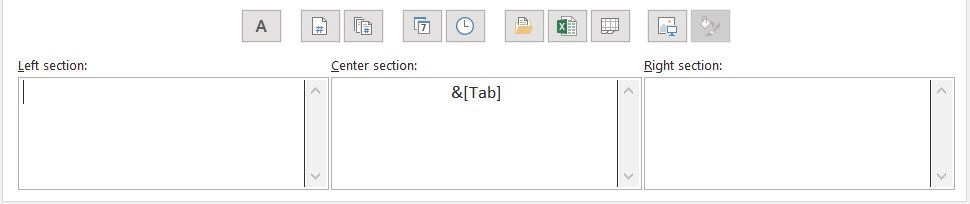
\includegraphics[width=\maxwidth{.95\linewidth}]{gfx/ch06_fig15}
	\caption{Insert Worksheet Name}
	\label{06:fig15}
\end{figure}

\textit{Print Preview} clarifies that the \textit{Expenses Summary} worksheet is not set to print correctly since part of the chart appears on a second page. \textit{Scaling} will correct this error, but only the \textit{Expenses Summary} worksheet should be rescaled.

\begin{enumbox}
	\begin{enumerate}
		\item Exit \textit{Print Preview} by clicking the arrow button in the top left corner.
		\item Ungroup the worksheets.
		\item If needed, click the \fmtWorksheet{Expenses Summary} worksheet tab to activate it.
		\item Click \fmtButton{Page Layout $ \Rightarrow $ Scale to Fit $ \Rightarrow $ Width Down-Arrow}. Select $ 1 $ page. This has the same result as selecting \fmtButton{Fit All Columns on One Page} in the \textit{Scaling} setting in \textit{Print Preview} (see Figure \ref{06:fig16}).
	\end{enumerate}
\end{enumbox}

\begin{figure}[H]
	\centering
	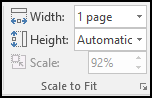
\includegraphics[width=\maxwidth{.35\linewidth}]{gfx/ch06_fig16}
	\caption{Scale to Fit}
	\label{06:fig16}
\end{figure}

\begin{enumbox}
	\begin{enumerate}
		\item Click \fmtButton{File $ \Rightarrow $ Print}.
		\item Confirm that the \fmtWorksheet{Expenses Summary} worksheet is now printing on one page only. There should only be $ 13 $ pages in the printout.
		\item Exit \textit{Print Preview}.
		\item Save the \fmtWorksheet{CH6-2017 Personal Budget} workbook.
		\item Compare the workbook with the self-check answer key (\fmtWorksheet{CH6-2017 Personal Budget Solution}) and then close and submit the \fmtWorksheet{CH6-2017 Personal Budget} workbook as directed by the instructor.
	\end{enumerate}
\end{enumbox}
	
\begin{center}
	\begin{tkwbox}{Key Take-Aways}
		\textbf{Printing}
		\\
		\begin{itemize}
			\setlength{\itemsep}{0pt}
			\setlength{\parskip}{0pt}
			\setlength{\parsep}{0pt}
			
			\item To print all the worksheets in a workbook at one time select \textit{Print Entire Workbook} in the \textit{Print Settings}.
			\item Page setup options, such as scaling, orientation, and headers/footers, can be applied to multiple worksheets at one time by grouping them.
			
		\end{itemize}
	\end{tkwbox}
\end{center}

\section{Chapter Practice}

\subsection{A Multiple Worksheet Template for a Sports Team}

The \textit{Pacific Northwest Soccer Club} coaches want team statistics consistently tracked. To help with this, create a template for season stats for each team. The \textit{High Flyers} team coach will use the template to enter that team's statistics into a workbook.

\begin{enumbox}
	\begin{enumerate}
		\item Open the data file \fmtWorksheet{PR6-Data} and save the file as \fmtWorksheet{PR6-Pacific NW Sports Team}.
		\item On the \fmtWorksheet{Season Stats} worksheet, copy \fmtLoc{A8:F19} to the same range in the \fmtWorksheet{Player Stats} worksheet.
		\item Group the worksheets and add the following formulas to both worksheets.
	
		\begin{itemize}
			\item In \fmtLoc{B19}, enter \fmtTyping{=COUNTA(B9:B18)} to count the number of \textit{X's} in those rows for children who played that game.
			\item Copy \fmtLoc{B19} to \fmtLoc{C19} to count the number of \textit{X's} in those rows for children who started the game.
			\item In \fmtLoc{D19}, enter \fmtTyping{=SUM(D9:D18)} to calculate the total number of shots taken. 
			\item Copy \fmtLoc{D19} to \fmtLoc{E19} to calculate the total number of goals.
			\item In \fmtLoc{F9}, calculate \textit{Goal Percentage} by dividing the number of \textit{Goals} by the number of \textit{Shots}. This calculation will display an error message because there are zeros in \fmtLoc{Column D}. An \fmtTyping{IF} statement that tests the value of \fmtLoc{Column D} will keep error messages from appearing. Change \fmtLoc{F9} to an \fmtTyping{IF} formula using the following three parameters.
			\begin{itemize}
				\item \textbf{Test}: is \fmtLoc{D9} greater than zero
				\item \textbf{If the Test is True}: the number of \textit{Goals} divided by the number of \textit{Shots}
				\item \textbf{If the Test is False}: zero
			\end{itemize}
			\item Copy \fmtLoc{F9} to \fmtLoc{F10:F19}.
			\item Format \fmtLoc{F9:F19} as percentages.
			\item Using \fmtButton{Home $ \Rightarrow $ Font $ \Rightarrow $ Fill Color}, set \fmtLoc{Row 10}, \fmtLoc{Row 12}, \fmtLoc{Row 14}, \fmtLoc{Row 16}, and \fmtLoc{Row 18} to \textit{No Fill}. 
			\end{itemize}	
		
		\item Ungroup the worksheets.
		\item Compare the workbook with the self-check answer key (\fmtWorksheet{PR6-Pacific NW Sports Team Solution}) and then save the file as a template called \fmtWorksheet{PR6-Pacific NW Team Template}. Make sure to save the  template to a USB drive and not the default folder for templates on the local hard drive.
		\item Make a new file using the \fmtWorksheet{PR6 Pacific NW Team Template} and save it as a regular Excel workbook named \fmtWorksheet{PR6-High Flyers}. 
		\item In the \fmtWorksheet{Season Stats} worksheet, enter the following data:
		
		\begin{itemize}
			\item \fmtLoc{C2} – High Flyers
			\item \fmtLoc{C3} – Fall and the current year (\ie Fall 2020)
			\item \fmtLoc{C4} – Pacific Northwest Soccer
		\end{itemize}
		
		\item Make up a coach's name, phone number, and email address for row $ 6 $.
		\item Make four copies of the \fmtWorksheet{Player Statistics} worksheet. Rename the player worksheets \fmtWorksheet{Player 1}, \fmtWorksheet{Player 2}, \fmtWorksheet{Player 3}, \fmtWorksheet{Player 4}, and \fmtWorksheet{Player 5}.
		\item Group all five \textit{Player} worksheets.
		\item Click cell \fmtLoc{C2} and enter \fmtTyping{='Season Stats'!C2}.
		\item Copy \fmtLoc{C2} to \fmtLoc{C3:C4}.
		\item Ungroup the worksheets.
		\item Click the \fmtWorksheet{Player 1} worksheet tab to activate it. 
		\item In cell \fmtLoc{C5}, enter the \textit{Player Name}: \fmtTyping{Juan Ramirez}. 
		\item Enter other data from Table \ref{06:tab03}:
	\end{enumerate}
\end{enumbox}
	
\begin{table}[H]
	\rowcolors{1}{}{tablerow} % zebra striping background
	{\small
		%\fontsize{8}{10} \selectfont %Replace small for special font size
		\begin{longtable}{L{0.65in}C{0.45in}C{0.50in}C{0.40in}C{0.40in}} %Left-aligned, Max width: 4.25in
			\textbf{Game} & \textbf{Played} & \textbf{Started} & \textbf{Shots} & \textbf{Goals}\endhead
			\hline
			Game $ 1  $  & X & X & $ 2 $ & $ 1 $ \\
			Game $ 2  $  & X & X & $ 3 $ & $ 1 $ \\
			Game $ 3  $  &   &   &       &       \\
			Game $ 4  $  & X & X &       &       \\
			Game $ 5  $  & X & X & $ 2 $ & $ 0 $ \\
			Game $ 6  $  & X & X &       &       \\
			Game $ 7  $  & X & X &       &       \\
			Game $ 8  $  & X & X & $ 1 $ & $ 1 $ \\
			Game $ 9  $  & X & X & $ 4 $ & $ 2 $ \\
			Game $ 10 $  & X & X & $ 3 $ & $ 3 $ \\
			\rowcolor{captionwhite}
			\caption{Player 1 Worksheet}
			\label{06:tab03}
		\end{longtable}
	}
\end{table}

\begin{enumbox}
	\begin{enumerate}
		\item Save the \fmtWorksheet{PR6-High Flyers} workbook.
		\item Click the \fmtWorksheet{Player 2} worksheet tab to activate it. 
		\item In cell \fmtLoc{C5}, enter the \textit{Player Name}: \fmtTyping{Zach Johnson}. 
		\item Enter other data from Table \ref{06:tab04}:
	\end{enumerate}
\end{enumbox}

\begin{table}[H]
	\rowcolors{1}{}{tablerow} % zebra striping background
	{\small
		%\fontsize{8}{10} \selectfont %Replace small for special font size
		\begin{longtable}{L{0.65in}C{0.45in}C{0.50in}C{0.40in}C{0.40in}} %Left-aligned, Max width: 4.25in
			\textbf{Game} & \textbf{Played} & \textbf{Started} & \textbf{Shots} & \textbf{Goals}\endhead
			\hline
			Game $ 1 $  & X & X & $ 1 $ & $ 1 $ \\
			Game $ 2 $  & X & X & $ 2 $ & $ 1 $ \\
			Game $ 3 $  & X &   & $ 1 $ & $ 1 $ \\
			Game $ 4 $  & X & X & $ 1 $ & $ 1 $ \\
			Game $ 5 $  & X & X & $ 2 $ & $ 0 $ \\
			Game $ 6 $  & X & X & $ 5 $ & $ 2 $ \\
			Game $ 7 $  & X & X & $ 4 $ & $ 2 $ \\
			Game $ 8 $  & X & X & $ 1 $ & $ 1 $ \\
			Game $ 9 $  & X & X & $ 4 $ & $ 1 $ \\
			Game $ 10 $ & X & X & $ 3 $ & $ 2 $ \\
			\rowcolor{captionwhite}
			\caption{Player 2 Worksheet}
			\label{06:tab04}
		\end{longtable}
	}
\end{table}

\begin{enumbox}
	\begin{enumerate}
		\item Save the \fmtWorksheet{PR6-High Flyers} workbook.
		
		\item Click the \fmtWorksheet{Player 3} worksheet tab to activate it. 
		\item In cell \fmtLoc{C5}, enter the \textit{Player Name}: \fmtTyping{Vito Lawrenz}. 
		\item Enter other data from Table \ref{06:tab05}:
	\end{enumerate}
\end{enumbox}
	
\begin{table}[H]
	\rowcolors{1}{}{tablerow} % zebra striping background
	{\small
		%\fontsize{8}{10} \selectfont %Replace small for special font size
		\begin{longtable}{L{0.65in}C{0.45in}C{0.50in}C{0.40in}C{0.40in}} %Left-aligned, Max width: 4.25in
			\textbf{Game} & \textbf{Played} & \textbf{Started} & \textbf{Shots} & \textbf{Goals}\endhead
			%\hline
			Game $ 1  $ & X & X & $ 0 $ & $ 0 $ \\
			Game $ 2  $ & X & X & $ 1 $ & $ 1 $ \\
			Game $ 3  $ & X & X & $ 2 $ & $ 0 $ \\
			Game $ 4  $ & X &   & $ 1 $ & $ 1 $ \\
			Game $ 5  $ & X & X & $ 2 $ & $ 0 $ \\
			Game $ 6  $ & X & X & $ 3 $ & $ 1 $ \\
			Game $ 7  $ & X & X & $ 2 $ & $ 1 $ \\
			Game $ 8  $ & X & X & $ 1 $ & $ 1 $ \\
			Game $ 9  $ & X & X & $ 1 $ & $ 1 $ \\
			Game $ 10 $ & X & X & $ 1 $ & $ 1 $ \\
			\rowcolor{captionwhite}
			\caption{Player 3 Worksheet}
			\label{06:tab05}
		\end{longtable}
	}
\end{table}

\begin{enumbox}
	\begin{enumerate}
		\item Save the \fmtWorksheet{PR6-High Flyers} workbook.
		\item Make up information for the names and data in the \fmtWorksheet{Player 4} and \fmtWorksheet{Player 5} worksheets.
		\item Click the \fmtWorksheet{Season Stats} worksheet to activate it.
	
		\item Click cell \fmtLoc{B9}. 
		\item Enter a $ 3 $-D formula to \fmtTyping{COUNTA} in \fmtLoc{B9} on worksheets \fmtWorksheet{Player 1} through \fmtWorksheet{Player 5}. 
		\item Copy \fmtLoc{B9} to \fmtLoc{B10:B18}.
		\item Copy \fmtLoc{B9} to \fmtLoc{C9:C18}.
		\item Change the formulas in \fmtLoc{B19} and \fmtLoc{C19} from \fmtTyping{COUNTA} to \fmtTyping{SUM}.
		\item Click cell \fmtLoc{D9}. 
		\item Enter a $ 3 $-D formula to \fmtTyping{SUM} cells \fmtLoc{D9} on worksheets \fmtWorksheet{Player 1} through \fmtWorksheet{Player 5}. 
		\item Copy \fmtLoc{D9} to \fmtLoc{D10:D18}.
		\item Copy \fmtLoc{D9} to \fmtLoc{E9:E18}.
		\item Using \fmtButton{Home $ \Rightarrow $ Font $ \Rightarrow $ Fill Color}, set \fmtLoc{Row 10}, \fmtLoc{Row 12}, \fmtLoc{Row 14}, \fmtLoc{Row 16}, and \fmtLoc{Row 18} to \textit{No Fill}. 
		\item Click \fmtButton{File $ \Rightarrow $ Print} to preview the worksheets in \textit{Print Preview}. Notice that only part of the data is printed for each worksheet since a \textit{Print Area} was incorrectly set when the file was first created. This print area needs to be cleared for each worksheet individually (modifying print areas cannot be done on grouped worksheets). 
		\item Exit \textit{Print Preview} by clicking the arrow in the top left corner of the screen. 
		\item Click the tab to activate each of the six worksheets one at a time, and then click \fmtButton{Page Layout $ \Rightarrow $ Page Setup $ \Rightarrow $ Print Area $ \Rightarrow $ Clear Print Area} for each worksheet.
		\item Click \fmtButton{File $ \Rightarrow $ Print} to preview the worksheets in \textit{Print Preview}. Notice that now all six sheets print correctly.
		\item Save the \fmtWorksheet{PR6-High Flyers} workbook.
		\item Compare the workbook with the self-check answer key (PR6-High Flyers Solution) and then close and submit the \fmtWorksheet{PR6-High Flyers} workbook and \fmtWorksheet{PR6-Pacific NW Team Template}.
	\end{enumerate}
\end{enumbox}
	
\section{Scored Assessment}

\subsection{A Multiple Worksheet Template for National Parks Data}

A template for National Parks usage data and a summary of the park's visitation data will be developed. To do this, create a template with a  summary and individual park worksheets and then use that template to enter park data for five national parks.

\begin{enumbox}
	\begin{enumerate}
		\item Open a new blank workbook.
		\item Change the name of \fmtWorksheet{Sheet1} to \fmtWorksheet{Park Data}. 
		\item Design a professional quality worksheet to display individual park data. Include areas to enter the name of a park and the park statistics as found in Tables \ref{06:tab06}, \ref{06:tab07}, and \ref{06:tab08} below. (\textit{Note}: do not copy the physical layout of the data tables.) Figure \ref{06:fig17} shows how this could be set up, though students are encouraged to explore alternate layouts. (\textit{Note}: the camping graphic is available in the student files as \textit{CH6-Camping.png}.)

		\begin{figure}[H]
			\centering
			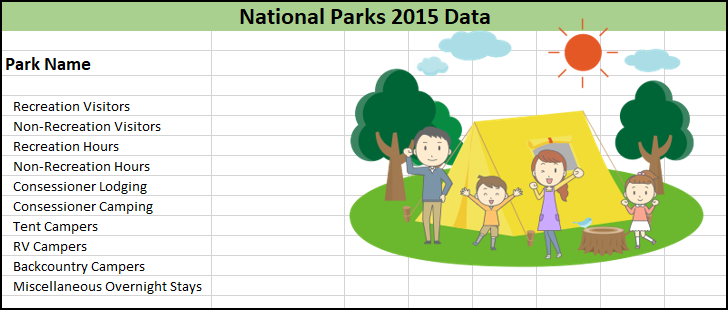
\includegraphics[width=\maxwidth{.95\linewidth}]{gfx/ch06_fig17}
			\caption{Sample setup}
			\label{06:fig17}
		\end{figure}

		\item Make a copy of the \fmtWorksheet{Park Data} worksheet and rename it \fmtWorksheet{Summary Park Data}. Make sure both worksheets are laid out the same. The \fmtWorksheet{Summary Park Data} worksheet tab should be first, and the \fmtWorksheet{Park Data} worksheet tab should be second.
		\item Save the file as a template called \fmtWorksheet{SC6-National Parks Template}. Make sure this gets saved to a USB drive and not the default template folder on the hard drive.
		\item Close \fmtWorksheet{SC6-National Parks Template}.
		\item Make a new file using the template and save it as a regular Excel workbook named \fmtWorksheet{SC6-Five National Parks}.
		\item Make four copies of the \fmtWorksheet{Park Data} worksheet. Rename the five \textit{Park Data} worksheets after the five parks listed in Table \ref{06:tab06}.\footnote{Note: The National Park $ 2015 $ Data is from: \url{https://irma.nps.gov/Stats/SSRSReports}.}
		\item Enter the park name in cell \fmtLoc{B3} on each of the \textit{Park Data} sheets.
		\item To make the sheets a bit more readable, right-align cell \fmtLoc{B3} on each of the \textit{Park Data} worksheets.
		\item Click cell \fmtLoc{A3} on the Summary Park Data worksheet. Enter \fmtTyping{Summary} into that cell.
		\item Enter the park data for each of the parks in the five worksheets.
	\end{enumerate}
\end{enumbox}
	
\begin{table}[H]
	\rowcolors{1}{}{tablerow} % zebra striping background
	{\small
		%\fontsize{8}{10} \selectfont %Replace small for special font size
		\begin{longtable}{L{1.25in}L{0.70in}L{0.60in}L{0.70in}L{0.60in}} %Left-aligned, Max width: 4.25in
		\textbf{Name} & \textbf{Recreation Visitors} & \textbf{Non-recreation Visitors} & \textbf{Recreation Hours} & \textbf{Non-recreation Hours} \endhead
		\hline
		Acadia NP       & $ 2,811,184 $  & $ 47,100 $    & $ 14,452,151 $ & $ 47,100 $    \\
		Blue Ridge PKWY & $ 15,054,603 $ & $ 1,942,260 $ & $ 93,977,122 $ & $ 971,136 $   \\
		Crater Lake NP  & $ 614,712 $    & $ 49,600 $    & $ 4,033,484 $  & $ 24,800 $    \\
		Yellowstone NP  & $ 4,097,710 $  & $ 1,156,118 $ & $ 82,016,845 $ & $ 711,795 $   \\
		Yosemite NP     & $ 4,150,217 $  & $ 155,081 $   & $ 78,505,877 $ & $ 3,993,223 $ \\
		\rowcolor{captionwhite}
		\caption{National Park Data, Pt 1}
		\label{06:tab06}
		\end{longtable}
	}
\end{table}

\begin{table}[H]
	\rowcolors{1}{}{tablerow} % zebra striping background
	{\small
		%\fontsize{8}{10} \selectfont %Replace small for special font size
		\begin{longtable}{L{1.25in}L{0.60in}L{0.60in}L{0.60in}L{0.60in}} %Left-aligned, Max width: 4.25in
			\textbf{Name} & \textbf{Concessioner Lodging} & \textbf{Concessioner Camping} & \textbf{Tent Campers} & \textbf{RV Campers} \endhead
			\hline
			Acadia NP       & $ 0 $       & $ 0 $       & $ 135,000 $ & $ 32,094 $  \\
			Blue Ridge PKWY & $ 53,688 $  & $ 0 $       & $ 61,481 $  & $ 33,499 $  \\
			Crater Lake NP  & $ 34,629 $  & $ 55,596 $  & $ 7,548 $   & $ 0 $       \\
			Yellowstone NP  & $ 552,940 $ & $ 584,979 $ & $ 104,149 $ & $ 69,830 $  \\
			Yosemite NP     & $ 938,418 $ & $ 0 $       & $ 588,701 $ & $ 284,372 $ \\
			\rowcolor{captionwhite}
			\caption{National Park Data, Pt 2}
			\label{06:tab07}
		\end{longtable}
	}
\end{table}

\begin{table}[H]
	\rowcolors{1}{}{tablerow} % zebra striping background
	{\small
		%\fontsize{8}{10} \selectfont %Replace small for special font size
		\begin{longtable}{L{1.25in}L{0.60in}L{0.60in}} %Left-aligned, Max width: 4.25in
			\textbf{Name} & \textbf{Backcountry Campers} & \textbf{Misc Overnight Stays} \endhead
			\hline
			Acadia NP       & $ 1,233 $   & $ 8,343 $  \\
			Blue Ridge PKWY & $ 2,101 $   & $ 1,294 $  \\
			Crater Lake NP  & $ 3,253 $   & $ 0 $      \\
			Yellowstone NP  & $ 44,898 $  & $ 11,715 $ \\
			Yosemite NP     & $ 211,966 $ & $ 39,214 $ \\
			\rowcolor{captionwhite}
			\caption{National Park Data, Pt 3}
			\label{06:tab08}
		\end{longtable}
	}
\end{table}

\begin{enumbox}
	\begin{enumerate}
		\item On each of the Park Data worksheets, apply comma format to \fmtLoc{B5:B14} and reduce the number of decimal places to zero.
		\item On the \fmtWorksheet{Summary Park Data} worksheet, create formulas for all the fields that sum the same fields in the five park worksheets. So, cell \fmtLoc{B5} on \fmtWorksheet{Summary Park Data} should contain a sum of the \textit{Recreation Visitors} for all five parks.
		\item On the \fmtWorksheet{Summary Park Data} worksheet, apply comma format to \fmtLoc{B5:B14} and reduce the number of decimal places to zero.
		\item Click \fmtButton{File $ \Rightarrow $ Print} and check the entire workbook in \textit{Print Preview} to ensure that it is printing professionally. Make any changes needed.
		\item Save the \fmtWorksheet{SC6-Five National Parks} workbook.
		\item Close and submit both the \fmtWorksheet{SC6-Five National Parks} and \fmtWorksheet{SC6-National Parks Template} files as directed by the instructor.
	\end{enumerate}
\end{enumbox}